\begin{frame}{Case Study}
    \begin{itemize}
        \item Suppose we split the class into two groups by drawing a line down the middle of the classroom.
        \item Let $\hat{p}_L$ be the proportion of students on the left side who own an Apple product.
        \item Let $\hat{p}_R$ be the proportion of students on the right side who own an Apple product.
    \end{itemize}
    Would you expect these two proportions to be \textit{exactly} the same?
\end{frame}

\begin{frame}{Case Study}
    \begin{itemize}
        \item There's no reason to believe that Apple users tend to sit on one side of the room or another*, so we would expect the proportions to be pretty similar.
        \item But we probably wouldn't expect these numbers to be exactly the same.
        \item This small expected variation is due to random chance.
    \end{itemize}
    
    \vspace{12pt}* What assumption are we making about how these variables relate to one another?
\end{frame}

\begin{frame}{Case Study: Malaria Vaccine}
    We consider a study on the malaria vaccine, PfSPZ. 
    \begin{itemize}
        \item Volunteer patients randomized into one of two experimental groups.
        \begin{itemize}
            \item 14 patients received the vaccine.
            \item 6 patients recieved a placebo.
        \end{itemize}
        \item After 19 weeks, all patients are exposed to a (drug-sensitive) strain of malaria.
    \end{itemize}
\end{frame}

\begin{frame}{Case Study: Malaria Vaccine}
    These are the results:
    \begin{center}
        \begin{tabular}{r l cc r}
		& & \multicolumn{2}{c}{{\texttt{outcome}}} & \\
        \cline{3-5}
		& & Infection & No Infection & Total  \\ 
        \cline{2-5}
        \multirow{2}{*}{{\texttt{treatment}}} 
        & Vaccine & 5 & 9 & 14  \\ 
  		& Placebo & 6 & 0 & 6  \\ 
        \cline{2-5}
  		& Total	& 11 & 9 & 20  \\
        \cline{2-5}
    \end{tabular}
    \end{center}
    This suggests infection rates of 35.7\% for the treatment group and 100\% for the control (placebo) group.
\end{frame}

\begin{frame}{Case Study: Malaria Vaccine}
    \begin{itemize}
        \item This study is an experiment, because treatment levels were assigned by the researchers.
        \item Therefore we can evaluate a causal relationship between the vaccine and incidence of malaria.
        \item It is not clear what level of blinding was used, but since they used a placebo, it is probably blind.
    \end{itemize}
\end{frame}

\begin{frame}{Strength of Evidence}
    \begin{itemize}
        \item We expect there to be some differences in our sample estimates, even if the true values are exactly equal. 
        \item The sample size is small, so it's not clear whether the vaccine would be effective in the population at large.
        \item It's impossible to know whether the observed difference is due to the vaccine's efficacy or random chance.
        \item It's possible that such a large difference is normal (due to chance alone) in such a small sample.
    \end{itemize}
    \vspace{12pt}\small Note: In reality, clinical trials suggest that PfSPZ is effective, but storage and transportation costs make it difficult to distribute to areas where malaria is prevalent.
\end{frame}

\begin{frame}{Variability in the Data}
    This is a good reminder that our observed data may not perfectly reflect the truth!
    \begin{itemize}
        \item This is due to \textbf{random noise}, the variability between values due to random chance.
        \item Random noise and sample size are things we take into account when statistically analyzing scientific claims.
    \end{itemize}
\end{frame}

\begin{frame}{Competing Claims}
    Whenever we ask a research question, we always have two competing claims, or \textbf{hypotheses}. These are labeled $H_0$ ("H-nought") and $H_A$ ("H-A").
    
    \vspace{12pt}$H_0$: \textbf{Independence model}. The variables treatment and outcome are independent. They have no relationship. Any observed difference between the proportion of patients who developed an infection in the two groups is due to chance.
    
    \vspace{12pt}$H_A$: \textbf{Alternative model}. The variables are not independent. The difference in infection rates is not due to chance. The vaccine affected the rate of infection.
\end{frame}

\begin{frame}{Independence Model}
    If $H_0$, the independence model, is true
    \begin{itemize}
        \item The vaccine is irrelevant to infection status.
        \item The 11 patients who developed an infection would have develop an infection regardless of which group they were assigned to.
        \item The 9 who did not develop an infection wouldn't have developed an infection regardless of which group they were assigned to.
        \item The difference in infection rates was due to chance alone.
    \end{itemize}
\end{frame}

\begin{frame}{Alternative Model}
    If $H_A$, the alternative model, is true
    \begin{itemize}
        \item Infection rates are influenced by whether or not a person received the vaccine.
    \end{itemize}
\end{frame}

\begin{frame}{Which Model is Correct?}
    We draw conclusions about which model is more likely to be true by assessing how strong our evidence is
    \begin{itemize}
        \item Do the data conflict with $H_0$ strongly enough to conclude $H_A$?
        \item This depends on
        \begin{enumerate}
            \item How different the groups are.
            \item How variable the groups are.
            \item How much data we have.
        \end{enumerate}
    \end{itemize}
\end{frame}

\begin{frame}{Simulations}
    We can start to think about the strength of our evidence using simulations.
    \begin{itemize}
        \item Our simulations will assume that our independence model is true.
        \item We want to know if it is common to see differences as large as the one we saw in our study.
        \item If it is common, it is more likely that the difference was due to random chance.
        \item If it is uncommon, it is more likely that the vaccine is helpful in preventing malaria.
    \end{itemize}
\end{frame}

\begin{frame}{Simulations}
    Simulations sound complicated, but the idea here is just to assume that the vaccine has no effect and then re-randomize the patients to the treatment and control groups.
    \begin{itemize}
        \item If the vaccine has no effect, we assume that the 11 patients who developed an infection would have done so no matter what. 
        \item We also assume that the 9 who did not develop an infection would have no infection no matter what.
    \end{itemize}
\end{frame}

\begin{frame}{Simulations}
    We can approach this simulation like this:
    \begin{enumerate}
        \item Take 20 note cards to represent the 20 patients \item Write each infection status on a note card (11 will say "infection"; 9 will say "no infection").
        \item Shuffle the note cards and then randomly pull out 14 for the \texttt{vaccine} pile. Put the other 6 into the \texttt{placebo} pile.
        \item Count up how many infections are in each pile.
    \end{enumerate}
\end{frame}

\begin{frame}{Simulations}
    Doing this once, we get
    \begin{center}
        \begin{tabular}{r l cc r}
		& & \multicolumn{2}{c}{{\texttt{outcome}}} & \\
        \cline{3-5}
		& & Infection & No Infection & Total  \\ 
        \cline{2-5}
        \multirow{2}{*}{{\texttt{treatment}}} 
        & Vaccine & 7 & 7 & 14  \\ 
  		& Placebo & 4 & 2 & 6  \\ 
        \cline{2-5}
  		& Total	& 11 & 9 & 20  \\
        \cline{2-5}
    \end{tabular}
    \end{center}
    Here, there is an infection rate of 50\% for the treatment group and 66.6\% in the placebo group, a difference of 16.7\%. This is much smaller than in the actual study!
\end{frame}

\begin{frame}{Checking For Independence}
    The real power of simulations comes from repetition. Using \texttt{R}, I repeated this simulation 10,000 times. 
    \begin{center}
        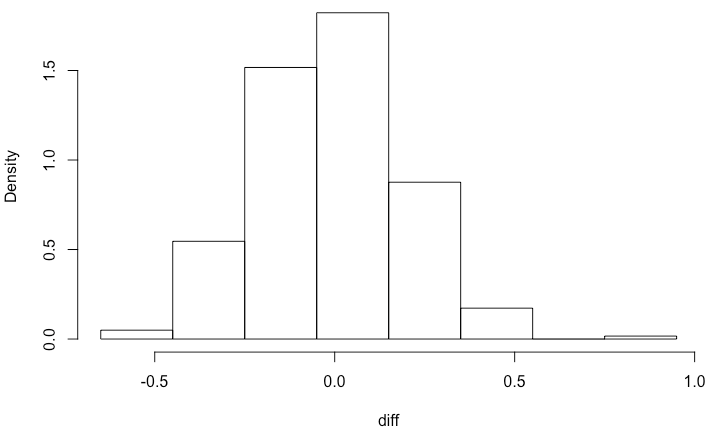
\includegraphics[scale=0.3]{images/diffhist.png}
    \end{center}
    Histogram of the differences across 10,000 repetitions.
\end{frame}

\begin{frame}{Checking For Independence}
    \begin{itemize}
        \item In the actual study, the difference in infection rates was 64.3\%.
        \item In my simulations, the average difference was only 0.06\%.
        \item I found a difference as big as the one in the study only 33 times.
        \begin{itemize}
            \item This means that, if the vaccine is not useful, a difference of 64.3\% happens by chance less than 1\% of the time!
        \end{itemize}
        \item This suggests that we have pretty good information despite the small sample size.
    \end{itemize}
\end{frame}

\begin{frame}{Moving Forward}
    The concepts we've been talking about with our case study are what we want to get at with this course!
    \begin{itemize}
        \item Hypotheses
        \item Testing claims (testing for independence)
        \item Figuring out how uncertain we are about our results
    \end{itemize}
    Eventually, we will formalize these concepts and talk about how to test our claims without simulations.
\end{frame}

\begin{frame}{A Note About R Code}
    I've been using a lot of code to write these slides!
    \begin{itemize}
        \item I've added a new page to the course website that will contain links to all of this R code.
        \item This code will be heavily commented to make it easier to follow and I will set it up so that you will not need to download any additional data.
        \item As always, learning R is completely optional, but the code is there if you're interested.
    \end{itemize}
\end{frame}